\documentclass[11pt]{amsart}

\usepackage[top=25mm, bottom=25mm, left=25mm, right=25mm]{geometry}
\usepackage{amsmath,amssymb,amsthm}
\usepackage{enumitem}
\usepackage[dvipsnames]{xcolor}
\usepackage{graphicx}
\usepackage{wrapfig}
\usepackage{capt-of}
\usepackage{tikz}
\usetikzlibrary{calc,positioning,decorations.pathreplacing,arrows.meta}
\usepackage{url}
\usepackage[hidelinks]{hyperref}
\usepackage[none]{hyphenat}
\raggedbottom

\tikzset{vertex/.style={circle,draw=black,fill=black,inner sep=0,minimum size=5pt,text=white,font=\footnotesize}}

\newtheorem{theorem}{Theorem}[section]
\newtheorem{lemma}[theorem]{Lemma}
\newtheorem{corollary}[theorem]{Corollary}
\newtheorem{claim}[theorem]{Claim}
\newtheorem{proposition}[theorem]{Proposition}
\newtheorem{conjecture}[theorem]{Conjecture}
\newtheorem{question}[theorem]{Question}
\newtheorem{problem}[theorem]{Problem}
\newtheorem*{theorem*}{Theorem}

\theoremstyle{definition}
\newtheorem{definition}[theorem]{Definition}
\newtheorem{remark}[theorem]{Remark}

\newenvironment{claimproof}{%
  \renewcommand{\qedsymbol}{$\boxdot$}%
  \begin{proof}%
}{%
  \end{proof}%
}

\newlist{lemenum}{enumerate}{1}
\setlist[lemenum]{label=(\roman*), ref=\thelemma(\roman*)}

\newcommand{\eps}{\varepsilon}
\newcommand{\ex}{\mathrm{ex}}
\newcommand{\Hom}{\mathrm{Hom}}
\newcommand{\Pb}{\mathbb{P}}
\newcommand{\bE}{\mathbb{E}}
\newcommand{\bF}{\mathbb{F}}
\newcommand{\bR}{\mathbb{R}}
\newcommand{\bZ}{\mathbb{Z}}
\newcommand{\cD}{\mathcal{D}}
\newcommand{\cF}{\mathcal{F}}
\newcommand{\cG}{\mathcal{G}}
\newcommand{\cH}{\mathcal{H}}
\newcommand{\cT}{\mathcal{T}}
\DeclareMathOperator{\Var}{Var}
\DeclareMathOperator{\polylog}{polylog}

\title{Polynomial bounds for quasiplanar graphs}
\author{Aleksa Milojevi\'c}
\author{Patryk Morawski}
\author{Benny Sudakov}
\thanks{AM, PM, BS: Department of Mathematics, ETH Z\"urich, Switzerland. Email: {\tt \char`\{aleksa.milojevic, patryk.morawski, benjamin.sudakov\char`\}@math.ethz.ch}. Research supported in part by SNSF grant 200021-228014.}
\author{Istv\'an Tomon}
\thanks{IT: Ume\r{a} University, Sweden. Email: {\tt istvantomon@gmail.com}. Research supported in part by the Swedish Research Council grant VR 2023-03375.}
\date{}

\begin{document}

\sloppy 
\begin{abstract}
A graph $G$ is $k$-quasiplanar if it can be drawn in the plane without $k$ pairwise crossing edges. It was a longstanding conjecture that $n$-vertex $k$-quasiplanar graphs have $O_k(n)$ edges. This was recently resolved by Sadhu and, independently, by Pach, Tardos, and Zeng, based on a theorem in topology proven by Beeker and Lazarovich. These papers showed that $k$-quasiplanar graphs have at most $k^{O(k)}n$ edges.

In this note, we greatly improve the dependence on $k$ and show that every $k$-quasiplanar $n$-vertex graph has at most $O(k^2n)$ edges. The proof is based on a geometric charging scheme and Erd\H{o}s-Szekeres type combinatorial arguments.
\end{abstract}

\maketitle

\vspace{-0.7cm}

\section{Introduction}

A graph $G$ is \textit{planar} if it can be drawn in the plane with no two edges crossing. Planar graphs are among the most extensively studied graph families, both from a structural and an algorithmic perspective. A beautiful theorem of F\'ary \cite{Fary} (first proved by Wagner in 1936) is that every planar graph can be drawn in the plane with straight line segments as edges. Moreover, it follows from Euler's polyhedral formula that the maximum number of edges of an $n$-vertex planar graph is at most $3n-6$, which is optimal. This bound puts a heavy restriction on which graphs can be drawn without crossings.

A natural relaxation of planarity was introduced in the early 1990's. A graph $G$ is \emph{$k$-quasiplanar} if it can be drawn in the plane such that no $k$ edges pairwise cross. Compared to planarity, which corresponds to the case $k=2$, $k$-quasiplanarity is much less understood for $k\geq 3$. The difficulty of this notion stems from the fact that  3-quasiplanar graphs can already exhibit strange behavior. For example, Brandenburg \cite{Brandenburg} showed that the complete graph $K_{10}$ is 3-quasiplanar, however, it has no 3-quasiplanar drawing with straight line segments. Furthermore, Ackerman and Tardos \cite{AT} showed that there exist $3$-quasiplanar graphs such that in every 3-quasiplanar drawing, there are pairs of edges that cross more than once.

In the past three decades, the following question became one of the central problems in the theory of graph drawings.
\smallskip
\begin{quote}\centering
\textit{What is the maximum number of edges of an $n$-vertex $k$-quasiplanar graph?  }
\end{quote}
\smallskip

In 1996, Pach, Shahrokhi, and Szegedy \cite{PSSz} conjectured that for every fixed $k$, this maximum is $O_k(n)$, and this conjecture was later reiterated by Brass, Moser and Pach \cite{BMP}. The lack of very dense constructions of $k$-quasiplanar graphs led to an even more ambitious folklore conjecture that the above maximum is $O(kn)$. These conjectures proved to be very influential and played an important role in the development of modern combinatorial geometry. The attempts to resolve them led to a large number of different geometric and combinatorial techniques, including divide-and-conquer arguments, the use of partial orders, ordered graphs, and Davenport-Schinzel sequences, Ramsey-type arguments, charging schemes, and balanced separators. 

We now give a (far from complete) overview of the history of results towards these conjectures. The $k=3$ case was confirmed by Agarwal, Aronov, Pach, Pollack, and Sharir \cite{AAPPS} just a year later, and Ackerman and Tardos \cite{AT} proved that the maximum is between $7n-O(1)$ and $8n-20$. The $k=4$ case was then confirmed by Ackerman \cite{Ackerman} in 2009. In general, the quasi-linear upper bound $O(n(\log n)^{2k-4})$ was proved by Pach, Shahrokhi, and Szegedy \cite{PSSz}, which was later improved to $n(\log n)^{O(\log k)}$ by Fox and Pach \cite{FP}. Until recently, the best known bound $n(\log n/\log k)^{O(\log k)}$ was due to Fox, Pach, and Suk \cite{FPS}. A notable corollary of this result is that if $G$ is an $n$-vertex graph with at least $n^{1+\delta}$ edges, then any drawing of $G$ contains at least $n^{\eps}$ pairwise crossing edges for some $\eps=\eps(\delta)>0$.

The difficulty of the above conjectures led researchers to consider special drawings, which also proved to be quite difficult. The only fully understood case concerns drawings where the points are in convex position, and edges are straight line segments. In this case, Capoyleas and Pach \cite{CP} proved that the maximum number of edges is exactly $2(k-1)n - \binom{2k-1}{2}$. In the less restricted case, when the edges are straight-line segments or $x$-monotone curves (and there is no assumption on the vertices), Valtr \cite{Valtr,Valtr2} proved the bound $O_k(n\log n)$. Furthermore, the sharper bound $O(k^2n\log n)$ for straight line drawings follows from a work of T\'oth \cite{Toth}.

The linear upper bound $O_k(n)$ for the maximum number of edges of $k$-quasiplanar graphs was finally established in recent works of Sadhu \cite{Sadhu} and Pach, Tardos, and Zeng \cite{PTZ}. More precisely, it was independently discovered that this bound essentially follows from a topological result of Beeker and Lazarovich \cite{BL} from 2017. Since their work uses terminology quite different from that familiar to combinatorial geometers, and Beeker and Lazarovich were likely unaware of the quasiplanar graph conjecture, the connection remained unnoticed until it was uncovered with the help of large language models. The explicit bound $k^{(2+o(1))k} n$ is also established in \cite{PTZ}, where the authors note that the dependence on $k$ is unlikely to be sharp.

Building on these recent works, we greatly improve the dependence on $k$, and show the upper bound $O(k^2n)$. This quantitatively improves all previous results for sufficiently large $k=k(n)$, even the bounds that only apply for the special case of straight line drawings. Our proof is also combinatorial and self-contained. As we were preparing to post this article, we have learned that, independently from our work, an updated version of Sadhu's work \cite{Sadhu} on arXiv also claims the improved $O(k^2n)$ bound.

\begin{theorem}\label{thm:main}
Let $G$ be a $k$-quasiplanar $n$-vertex graph. Then $G$ has at most $O(k^2n)$ edges.
\end{theorem}

This theorem has an interesting corollary for drawings of complete graphs as well. Somewhat surprisingly, the following simple question is already poorly understood. What is the minimum number of pairwise crossing edges in a straight line drawing of $K_n$? Aronov, Erd\H{o}s, Goddard, Kleitman, Klugerman, Pach, and Schulman \cite{AEGKKPS} proved in 1991 that every such drawing contains at least $\Omega(\sqrt{n})$ pairwise crossing edges, while it is conjectured (see e.g. \cite{BMP}) that the answer should be $\Omega(n)$. The currently best known lower bound $n^{1-o(1)}$ was established not long ago by Pach, Rubin, and Tardos \cite{PRT}. Since their proof heavily relied on the fact that the edges are drawn as straight line segments, the authors asked about the minimum number of pairwise crossings in arbitrary drawings of $K_n$. This problem is even less understood, and there is no known drawing of $K_n$ with fewer than linearly many pairwise crossing edges. The aforementioned result of Fox, Pach and Suk \cite{FPS} gives a lower bound of $n^{\Omega(1)}$. An immediate corollary of Theorem \ref{thm:main} sharpens this to $\Omega(n^{1/2})$ by taking $k=cn^{1/2}$ for a small constant $c$.

\section{The size of quasiplanar graphs}

The general idea of the proof of Theorem \ref{thm:main} is as follows. 
We fix a drawing of our graph $G$ in which no $k$ edges pairwise cross, and we enclose the drawing in a sufficiently large disk.
We then remove small neighborhoods of the vertices and (roughly speaking) triangulate the resulting region using $O(n)$ triangles. 
Each curve corresponding to an edge of $G$ starts at a vertex, traverses some triangles of this triangulation and finishes at another vertex of $G$. 
We define a charging rule that charges each curve to at least one of the edges or triangles it traverses. 
At the same time, using that in our drawing no $k$ edges pairwise cross, we show that the number of curves that are charged to any given edge or triangle is at most $O(k^2)$. 
This immediately implies that the number of edges of $G$ is at most $O(k^2)$ times the number of triangles in our triangulation, i.e., $O(k^2n)$.

\subsection{Setup.}
Formally, let $G$ be an $n$-vertex $k$-quasiplanar graph and fix a drawing of $G$ in which no $k$ edges pairwise cross. 
We identify the vertices of $G$ with the corresponding points in the plane, and the edges of $G$ with \emph{continuous curves}, i.e., the images of continuous functions $\phi:[0,1]\rightarrow \mathbb{R}^2$. 
A \emph{crossing} between two curves is an intersection point that is not an endpoint of any of the curves. We make a few standard non-degeneracy assumptions: no curve goes through a vertex, curves are non-self intersecting, and no two curves touch, i.e., if two curves cross then one curve passes to the other side of the other curve. 
It is well known that a drawing can be redrawn satisfying these assumptions without creating new crossing pairs.

To define our triangulation, around every vertex $v\in V(G)$ we draw a small generic triangle $T_v$ such that $T_v$ is disjoint from all curves whose endpoint is not $v$.
We can guarantee that any two of these triangles are disjoint, no curve passes through a vertex of $T_v$, and every curve crosses the boundary of $T_v$ at most once. 
Additionally, we draw a large triangle $T_0$ enclosing the whole drawing of $G$ and all these small triangles. Let $\cT$ be a triangulation of $T_0\setminus \big(\bigcup_{v\in V(G)} T_v\big)$, whose vertices are the vertices of the triangles $T_0$ and $T_v$, $v\in V(G)$. 
We call the drawings of the edges of $G$ \textit{curves}, in order to distinguish them from the edges of the triangulation $\cT$, which are called \textit{edges}. 
Figure~\ref{fig:triangulation} illustrates this construction.

\begin{wrapfigure}{r}{0.43\textwidth}
\centering
\setlength{\captionindent}{0pt}
\vspace{-0.22cm}

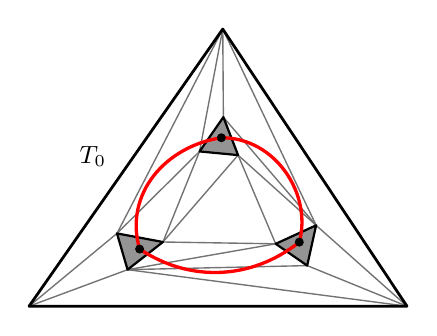
\begin{tikzpicture}[yscale=.55, xscale=0.6, line cap=round, line join=round, font=\small,
  edge/.style={line width=.5pt, draw=black!55},
  hole/.style={line width=.8pt, draw=black, fill=black!42},
  outer/.style={line width=1pt},
  curve/.style={draw=red, line width=1.2pt},
  gvertex/.style={circle, fill=black, inner sep=1.15pt}]
  \draw[edge] (0.000,0.000)--(1.861,1.681);
  \draw[edge] (0.000,0.000)--(2.085,0.844);
  \draw[edge] (1.861,1.681)--(3.609,3.574);
  \draw[edge] (1.861,1.681)--(4.100,6.400);
  \draw[edge] (2.085,0.844)--(5.220,1.441);
  \draw[edge] (2.085,0.844)--(5.887,0.938);
  \draw[edge] (2.085,0.844)--(8.000,0.000);
  \draw[edge] (2.834,1.483)--(3.609,3.574);
  \draw[edge] (2.834,1.483)--(4.424,3.489);
  \draw[edge] (2.834,1.483)--(5.220,1.441);
  \draw[edge] (3.609,3.574)--(4.100,6.400);
  \draw[edge] (4.100,6.400)--(4.113,4.366);
  \draw[edge] (4.100,6.400)--(6.076,1.868);
  \draw[edge] (4.113,4.366)--(6.076,1.868);
  \draw[edge] (4.424,3.489)--(5.220,1.441);
  \draw[edge] (4.424,3.489)--(6.076,1.868);
  \draw[edge] (5.887,0.938)--(8.000,0.000);
  \draw[edge] (6.076,1.868)--(8.000,0.000);
  \filldraw[hole] (2.834,1.483)--(1.861,1.681)--(2.085,0.844)--cycle;
  \filldraw[hole] (6.076,1.868)--(5.220,1.441)--(5.887,0.938)--cycle;
  \filldraw[hole] (4.113,4.366)--(3.609,3.574)--(4.424,3.489)--cycle;
  \draw[outer] (0.000,0.000)--(8.000,0.000)--(4.100,6.400)--cycle;
  \draw[curve] (2.340,1.320)..controls (3.400,0.550) and (4.700,0.600)..(5.720,1.480);
  \draw[curve] (5.720,1.480)..controls (6.000,2.600) and (5.200,3.900)..(4.070,3.890);
  \draw[curve] (4.070,3.890)..controls (2.900,3.700) and (2.000,2.600)..(2.340,1.320);
  \node[gvertex] at (2.340,1.320) {};
  \node[gvertex] at (5.720,1.480) {};
  \node[gvertex] at (4.070,3.890) {};
  \node at (1.35,3.45) {$T_0$};
\end{tikzpicture}
\caption{To obtain the triangulation $\cT$, we cut out sufficiently small triangles around each vertex of $G$, enclose the whole region in a big triangle and triangulate it.}
\label{fig:triangulation}
\end{wrapfigure}

A generic choice of triangles also ensures that no crossing between two curves is contained on an edge of $\cT$, and no curve touches an edge of $\cT$. Furthermore, we observe that $\cT$ has $3n+3$ vertices, $9n+3=O(n)$ edges, and $5n+1=O(n)$ triangles. 
The edges of $\cT$ that are adjacent to only one triangle of $\cT$ are the \emph{boundary edges},  and edges contained in two triangles are the \emph{internal edges}. Note that every triangle of $\cT$ contains at most one boundary edge.

Before introducing the charging scheme, we justify one further non-degeneracy assumption about how the curves of $G$ interact with the triangulation $\mathcal{T}$.
Namely, we assume that whenever a curve enters a triangle through one of its edges then it cannot immediately leave it again through the same edge.
In other words, we show that we can redraw our graph so that no edge of $\cT$ contains consecutive intersection points of a curve.
The same statement can be found in \cite{PTZ}, but we include a detailed proof for completeness.

\begin{lemma}\label{lemma:cleaning}
The curves of $G$ can be redrawn without creating new crossing pairs, such that no curve $\alpha$ has two consecutive intersection points with edges of $\mathcal{T}$ lying on the same edge.  
\end{lemma}
\begin{proof}
Let $xyz$ be a triangle of $\cT$ and assume that a curve $\alpha$  crosses $xy$ at points $a$ and $b$, such that the part of $\alpha$ between $a$ and $b$, denoted by $\alpha_0$, is contained entirely in $xyz$. The subcurve $\alpha_0$ together with the segment $ab$ is a closed Jordan curve enclosing a region $L$, called a \emph{lune} (see Figure~\ref{fig:lune}). Among all lunes in the drawing, choose a lune $L$  that is inclusion-minimal. Since $L$ lies in a single triangle $xyz$ of $\cT$, its interior contains no vertex of the drawing.

Replace $\alpha$ by a curve $\alpha'$ running sufficiently close to $ab$ on
the opposite side of $xy$ from $L$. This removes the two crossings at $a,b$.
We claim that it creates no new crossing pair of curves. Indeed,
by choosing $\alpha'$ sufficiently close to $ab$, any curve $\beta$ meeting
$\alpha'$ must cross the interior of $ab$. If $\beta$ did not meet $\alpha$,
then, upon entering $L$ through $ab$, it could neither end inside $L$ nor
leave through $\alpha$. It would therefore have to leave through $ab$ again.
The part of $\beta$ between two successive such crossings would bound,
together with a subsegment of $ab$, a lune strictly contained in $L$, a
contradiction.

Thus, we can sequentially destroy inclusion-minimal lunes until none remains without creating new crossing pairs. This proves the lemma.
\end{proof}


\begin{figure}[htbp]
\vspace{0pt}\centering
\setlength{\captionindent}{0pt}

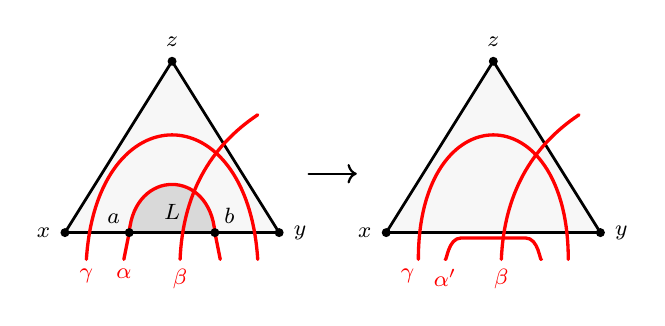
\begin{tikzpicture}[xscale=.68, yscale=.68, line cap=round, line join=round, font=\footnotesize,
  point/.style={circle,fill=black,inner sep=1.15pt},
  curve/.style={draw=red,line width=1.2pt}]

\begin{scope}
  \fill[black!3] (0,0)--(4,0)--(2,3.2)--cycle;
  \fill[black!15] (1.2,0)..controls (1.3,1.2) and (2.7,1.2)..(2.8,0)--cycle;
  \draw[line width=1pt] (0,0)--(4,0)--(2,3.2)--cycle;
  \draw[curve] (.4,-0.5)..controls (.6,2.6) and (3.4,2.6)..(3.6,-0.5);
  \draw[curve] (1.1,-0.5)..controls (1.1,-.5)..(1.2,0)..controls (1.3,1.2) and (2.7,1.2)..(2.8,0)..controls (2.9,-.5)..(2.9,-0.5);
  \draw[curve] (2.15,-0.5)..controls (2.2,.7) and (2.7,1.6)..(3.6,2.2);
  \node at (2,.38) {$L$};
  \node[text=red,below] at (1.1,-0.5) {$\alpha$};
  \node[text=red,below] at (2.15,-0.5) {$\beta$};
  \node[text=red,below] at (.4,-0.5) {$\gamma$};
  \node[point,label={[label distance=-2pt]above left:$a$}] at (1.2,0) {};
  \node[point,label={[label distance=-2pt]above right:$b$}] at (2.8,0) {};
  \node[point,label=left:$x$] at (0,0) {};
  \node[point,label=right:$y$] at (4,0) {};
  \node[point,label=above:$z$] at (2,3.2) {};
\end{scope}
\draw[->,line width=.8pt] (4.55,1.1)--(5.45,1.1);

\begin{scope}[xshift=6cm]
  \fill[black!3] (0,0)--(4,0)--(2,3.2)--cycle;
  \draw[line width=1pt] (0,0)--(4,0)--(2,3.2)--cycle;
  \draw[curve] (.6,-0.5)..controls (.6,2.6) and (3.4,2.6)..(3.4,-0.5);
  \draw[curve] (1.1,-0.5)..controls (1.13,-.55) and (1.15,-.1)..(1.4,-.1)--(2.6,-.1)..controls (2.85,-.1) and (2.87,-.55)..(2.9,-0.5);
  \draw[curve] (2.15,-0.5)..controls (2.2,.7) and (2.7,1.6)..(3.6,2.2);
  \node[text=red,below] at (1.1,-0.5) {$\alpha'$};
  \node[text=red,below] at (2.15,-0.5) {$\beta$};
  \node[text=red,below] at (.4,-0.5) {$\gamma$};
  \node[point,label=left:$x$] at (0,0) {};
  \node[point,label=right:$y$] at (4,0) {};
  \node[point,label=above:$z$] at (2,3.2) {};
\end{scope}
\end{tikzpicture}
\captionof{figure}{Removing an inclusion-minimal lune without introducing new crossings.}
\label{fig:lune}
\end{figure}

In the rest of the proof, we fix a drawing of $G$ satisfying the conclusion of Lemma \ref{lemma:cleaning}. 


\subsection{Left and right orders}
We now slowly move towards defining our charging rule, which charges each curve to at least one of the triangles or edges of $\cT$ it traverses.
Formally, we consider orientations of the edges of $\cT$ and write $\vec{xy}$ for the ordered pair $(x, y)$.
Then we can speak of the triangle lying on the left (or right) of a given $\vec{xy}$.
A crucial part of the charging scheme is to define, for every $\vec{xy}$, two associated linear orders, the left one $\prec_L$ and the right one $\prec_R$, each over the curves that cross this edge.
Since a given curve $\alpha$ may intersect $xy$ multiple times, we consider each such intersection separately.
More precisely, let
$$C_{xy}=\{(\alpha,p):\alpha\text{ is a curve intersecting }xy\text{ in point }p\},$$
and define $\prec_L$ and $\prec_R$ as linear orders on $C_{xy}$.

An informal meaning of these orders, which might be helpful to understand the upcoming definition is the following.
Assume that the curves $\alpha$ and $\beta$ do not intersect in our drawing.
Then $(\alpha, p) \prec_L (\beta, q)$ should mean that on the left of $\vec{xy}$ the curve $\alpha$ lies below $\beta$.
A key property that we will prove later, and which follows this intuition, is that if the relative orders of $(\alpha, p)$ and $ (\beta, q)$ are different on both sides, then the curves $\alpha$ and $\beta$ must cross.

\medskip

Formally, let $\vec{xy}$ be an oriented edge of $\cT$, and let $(\alpha,p),(\beta,q)\in C_{xy}$. We first order the pairs $(\alpha,p)$ and $(\beta,q)$ by $\prec_L=\prec_L^{xy}$, and later we argue that this definition indeed gives a linear order.

\begin{itemize}
    \item If $xy$ is a boundary edge with the only face of $\cT$ on the right side, then $(\alpha, p)\prec_L (\beta, q)$ if $p$ is closer to $x$ than $q$.
    \item Otherwise, let $xyz$ be the triangle of $\cT$ to the left of $\vec{xy}$. 
    Walk along the curves $\alpha$ and $\beta$ through the triangle $xyz$, starting from the points $p$ and $q$, and continuing until the first intersection with some side of the triangle.
    Let these intersection points be $p'$ and $q'$, respectively, and note that $p',q'\in xz\cup zy$ by the non-degeneracy assumption from Lemma~\ref{lemma:cleaning}. 
    We define the relation $\prec_L$ recursively depending on which of the following cases occurs (see also Figure~\ref{fig:left-order} for an illustration).
    \begin{itemize}
        \item If $p'\in xz$ and $q'\in zy$, then $(\alpha, p)\prec_L (\beta, q)$.\smallskip
        \item If $p'\in zy$ and $q'\in xz$, then $(\beta, q)\prec_L (\alpha, p)$.\smallskip
        \item If $p',q'\in xz$, then $(\alpha,p)$ and $(\beta,q)$ are ordered as $\prec_L^{xz}$ orders $(\alpha,p')$ and $(\beta,q')$.\smallskip
        \item If $p',q'\in zy$, then $(\alpha,p)$ and $(\beta,q)$ are ordered as $\prec_L^{zy}$ orders $(\alpha,p')$ and $(\beta,q')$.
    \end{itemize}
\end{itemize}

The right order $\prec_R$ is defined analogously, with the only difference being that we consider the triangles to the right of the edge $\vec{xy}$ instead of to the left.
We observe that left order of $\vec{xy}$ is the reverse of the right order of $\vec{yx}$, although we will not make use of this property. 

\medskip

\begin{figure}[htbp]
\centering

\begingroup

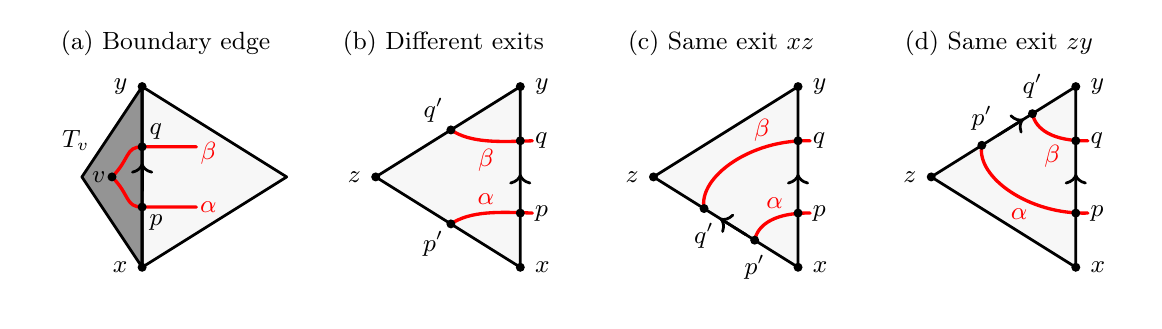
\begin{tikzpicture}[
  font=\small, line cap=round, line join=round,
  scale=.85,
  vertical diagram/.style={shift={(2.65,0)},rotate=90,scale=.9},
  point/.style={circle,fill=black,inner sep=1.15pt},
  note/.style={font=\scriptsize,align=center,text width=3.95cm,inner sep=0pt},
  heading/.style={font=\small,align=center}
]
\path[use as bounding box] (-.56,-.5) rectangle (15.96,3.58);
\begin{scope}
  \node[heading] at (1.5,3.35) {(a) Boundary edge};
  \begin{scope}[xscale=-1, xshift=-3.8cm, vertical diagram]
  \fill[black!3] (0,0)--(3,0)--(1.5,2.4)--cycle;
  \fill[black!42] (0,0)--(3,0)--(1.5,-1)--cycle;
  \draw[line width=1pt] (0,0)--(3,0)--(1.5,2.4)--cycle;
  \draw[line width=1pt] (0,0)--(3,0)--(1.5,-1)--cycle;
  \draw[line width=1pt, ->] (1.27,0)--(1.73,0);
  \draw[draw=red,line width=1.2pt] (1.5,-.5)..controls (1.2,-.2) and (1,-.28)..(1,0)..controls (1,.45) and (1,0.8)..(1,0.9);
  \draw[draw=red,line width=1.2pt] (1.5,-.5)..controls (1.8,-.2) and (2,-.28)..(2,0)..controls (2,.45) and (2,.9)..(2,0.9);
  \node[text=red] at (1,1.1) {$\alpha$};
  \node[text=red] at (1.9,1.1) {$\beta$};
  \node at (2.1,-1.1) {$T_v$};
  \node[point,label=left:$x$] at (0,0) {};
  \node[point,label=left:$y$] at (3,0) {};
  \node[point,label={[label distance=-3pt]below right:$p$}] at (1,0) {};
  \node[point,label={[label distance=-3pt]above right:$q$}] at (2,0) {};
  \node[point,label={[label distance=-3pt]left:$v$}] at (1.5,-.5) {};
  \end{scope}
\end{scope}

\begin{scope}[xshift=4.15cm]
  \node[heading] at (1.5,3.35) {(b) Different exits};
  \begin{scope}[vertical diagram]
  \fill[black!3] (0,0)--(3,0)--(1.5,2.4)--cycle;
  \draw[line width=1pt] (0,0)--(3,0)--(1.5,2.4)--cycle;
  \draw[line width=1pt, ->] (1.5,0)--(1.55,0);
  \draw[draw=red,line width=1.2pt] (.9,-0.2)..controls (.92,.35) and (.94,.82)..(.72,1.152);
  \draw[draw=red,line width=1.2pt] (2.1,-0.2)..controls (2.08,.35) and (2.06,.82)..(2.28,1.152);
  \node[text=red,above] at (.88,.57) {$\alpha$};
  \node[text=red,below] at (2.12,.57) {$\beta$};
  \node[point,label=right:$x$] at (0,0) {};
  \node[point,label=right:$y$] at (3,0) {};
  \node[point,label=left:$z$] at (1.5,2.4) {};
  \node[point,label=right:$p$] at (.9,0) {};
  \node[point,label=right:$q$] at (2.1,0) {};
  \node[point,label={[label distance=-3pt]below left:$p'$}] at (.72,1.152) {};
  \node[point,label={[label distance=-3pt]above left:$q'$}] at (2.28,1.152) {};
  \end{scope}
\end{scope}

\begin{scope}[xshift=8.3cm]
  \node[heading] at (1.5,3.35) {(c) Same exit $xz$};
  \begin{scope}[vertical diagram]
  \fill[black!3] (0,0)--(3,0)--(1.5,2.4)--cycle;
  \draw[line width=1pt] (0,0)--(3,0)--(1.5,2.4)--cycle;
  \draw[line width=1pt, ->] (1.5,0)--(1.55,0);
  \draw[line width=1pt, ->] (.54,.864)--(.81,1.296);
  \draw[draw=red,line width=1.2pt] (.9,-0.2)..controls (.91,.38) and (.71,.67)..(.45,.72);
  \draw[draw=red,line width=1.2pt] (2.1,-0.2)..controls (2.13,.78) and (1.5,1.66)..(.975,1.56);
  \node[text=red,above] at (.81,.39) {$\alpha$};
  \node[text=red] at (2.27,.6) {$\beta$};
  \node[point,label=right:$x$] at (0,0) {};
  \node[point,label=right:$y$] at (3,0) {};
  \node[point,label=left:$z$] at (1.5,2.4) {};
  \node[point,label=right:$p$] at (.9,0) {};
  \node[point,label=right:$q$] at (2.1,0) {};
  \node[point,label=below:$p'$] at (.45,.72) {};
  \node[point,label=below:$q'$] at (.975,1.56) {};
  \end{scope}
\end{scope}

\begin{scope}[xshift=12.45cm]
  \node[heading] at (1.5,3.35) {(d) Same exit $zy$};
  \begin{scope}[vertical diagram]
  \fill[black!3] (0,0)--(3,0)--(1.5,2.4)--cycle;
  \draw[line width=1pt] (0,0)--(3,0)--(1.5,2.4)--cycle;
  \draw[line width=1pt, ->] (1.5,0)--(1.55,0);
  \draw[line width=1pt, ->] (2.19,1.296)--(2.46,.864);
  \draw[draw=red,line width=1.2pt] (.9,-0.2)..controls (.87,.78) and (1.5,1.66)..(2.025,1.56);
  \draw[draw=red,line width=1.2pt] (2.1,-0.2)..controls (2.09,.38) and (2.29,.67)..(2.55,.72);
  \node[text=red,below] at (1.13,.94) {$\alpha$};
  \node[text=red,below] at (2.19,.39) {$\beta$};
  \node[point,label=right:$x$] at (0,0) {};
  \node[point,label=right:$y$] at (3,0) {};
  \node[point,label=left:$z$] at (1.5,2.4) {};
  \node[point,label=right:$p$] at (.9,0) {};
  \node[point,label=right:$q$] at (2.1,0) {};
  \node[point,label=above:$p'$] at (2.025,1.56) {};
  \node[point,label=above:$q'$] at (2.55,.72) {};
  \end{scope}
\end{scope}
\end{tikzpicture}
\endgroup

\caption{In the first two diagrams, we declare that $(\alpha, p)$ precedes $(\beta, q)$ in $\prec_L^{xy}$, while in the latter two diagrams, we copy the ordering from either $\prec_L^{xz}$ or $\prec_L^{zy}$.}
\label{fig:left-order}
\end{figure}


A priori, it is not obvious that the above definitions of $\prec_L^{xy}$ and $\prec_R^{xy}$ really give us linear orders. 
To address that, we will now give two alternative definitions of these orders.
The first immediately shows that  $\prec_L^{xy}$ and $\prec_R^{xy}$ are indeed linear orders, while the second is meant to give some intuition about how the orders arose in the first place.

\noindent
\begin{minipage}[t]{0.57\textwidth}
\setlength{\parindent}{\normalparindent}\indent
The first interpretation is that $\prec_L^{xy}$ can be seen as a lexicographic ordering of words defined as follows.
Let $\vec{xy}$ be an oriented edge, and let $(\alpha,p)\in C_{xy}$. Starting from $p$, start walking along $\alpha$ in the left direction of $\vec{xy}$. 
Every time we enter a triangle $x_0y_0z_0$ along an oriented edge $\vec{x_0y_0}$, orient  $x_0z_0$ as $\vec{x_0z_0}$, and orient $z_0y_0$ as $\vec{z_0y_0}$ (possibly reorienting previously oriented edges). 
If $\alpha$ leaves the triangle $x_0y_0z_0$ through $x_0z_0$ (informally, ``goes down"), we write the letter 0. If it leaves through $z_0y_0$ (informally, ``goes up"), we write down the letter 1. 
If we reach a boundary edge $\vec{x_0y_0}$, we write down the distance between $x_0$ and the intersection point of $\alpha$ with $x_0y_0$. 
This defines a word $w_{\alpha,p}^L$, whose letters are real numbers (see Figure~\ref{fig:word}). 
One can see that $\prec_{L}^{xy}$ corresponds to the \emph{lexicographic} ordering of these words, so $\prec_{L}^{xy}$ is indeed a linear order. 
We can treat $\prec_{R}^{xy}$ analogously, but we create a word $w^{R}_{\alpha,p}$ by traversing $\alpha$ in the right direction starting from $p$.\strut
\end{minipage}\hfill
\begin{minipage}[t]{0.4\textwidth}
\vspace{0pt}\centering
\setlength{\captionindent}{0pt}
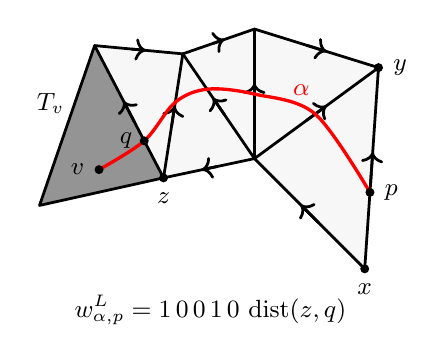
\begin{tikzpicture}[scale=.7, line cap=round, line join=round, font=\small,
  point/.style={circle,fill=black,inner sep=1.15pt},
  curve/.style={draw=red,line width=1.2pt}]
\coordinate (t0) at (1.00,4.05);
\coordinate (t1) at (2.60,3.90);
\coordinate (t2) at (3.90,4.35);
\coordinate (y)  at (6.15,3.65);
\coordinate (z)  at (2.25,1.65);
\coordinate (w)  at (3.90,2.00);
\coordinate (x)  at (5.90,0.00);
\coordinate (d)  at (0.00,1.15);
\coordinate (v)  at (1.08,1.80);
\coordinate (p)  at ($(x)!.38!(y)$);
\coordinate (q)  at ($(t0)!.72!(z)$);
\fill[black!42] (t0)--(d)--(z)--cycle;
\fill[black!3] (z)--(t0)--(t1)--(t2)--(y)--(x)--(w)--cycle;
\draw[line width=1pt] (t0)--(d)--(z);
\foreach \a/\b in {x/y, x/w, w/y, w/t2, t2/y, w/t1, t1/t2, w/z, z/t1, z/t0, t0/t1}{
  \draw[line width=1pt] (\a)--(\b);
  \draw[line width=1pt,->] ($(\a)!.42!(\b)$)--($(\a)!.58!(\b)$);
}
\draw[curve] plot[smooth,tension=.55] coordinates
  {(p) (5.0,2.81) (3.9,3.17) (3.05,3.26) (2.46,3.02) (q) (v)};
\node[text=red] at (4.75,3.25) {$\alpha$};
\node[point,label=below:$x$] at (x) {};
\node[point,label=right:$y$] at (y) {};
\node[point,label=below:$z$] at (z) {};
\node[point,label=right:$p$] at (p) {};
\node[point,label={[label distance=-1pt]left:$q$}] at (q) {};
\node[point,label=left:$v$] at (v) {};
\node at (.2,3.0) {$T_v$};
\node at (3.1,-.75) {$w^L_{\alpha,p}=1\,0\,0\,1\,0\,\operatorname{dist}(z,q)$};
\end{tikzpicture}
\captionof{figure}{To define the word $w^L_{\alpha, p}$ we walk along $\alpha$ from $p$ to the left of $\vec{xy}$. We write a $0$ when crossing a ``lower'' edge and a $1$ when crossing an ``upper'' edge. At a boundary edge of $\mathcal{T}$ we write the distance of the intersection points to the beginning of the edge.}
\label{fig:word}
\end{minipage}\par
\prevdepth=\dp\strutbox

\medskip

 Another way to think about the orders $\prec_L$ and $\prec_R$ is through the notion of universal covers. We will not use this perspective in any of the proofs, so we will describe it informally, with the hope that it would give the reader an intuitive understanding of the construction. A \textit{universal cover} of a topological space $X$ is a simply connected topological space $\widetilde{X}$ with a covering map $\pi:\widetilde{X}\to X$. For us, the universal cover is an infinite tree of triangles, and we denote it by $\widetilde{\cT}$. 

Let $e$ be an edge of $\widetilde{\cT}$ which projects to $xy$ and let $L$ be the set of all lifts $\widetilde{\alpha}$ of some curve $\alpha$ which have $\widetilde{\alpha}\cap e\neq \varnothing$. These correspond to the pairs $(\alpha, p)$ where $\alpha$ is a curve in $\cT$ and $p\in xy\cap \alpha$. Consider all triangles of $\widetilde{\cT}$ encountered by a lift of some edge intersecting $e$, and let their union be $D$. Since $D$ is a union of finitely many triangles in the infinite tree $\widetilde{\cT}$ and is connected, it is homeomorphic to a disc whose boundary contains $x$ and $y$. Therefore, $x$ and $y$ split the boundary of $D$ into two parts. Moreover, the lift of any curve $\alpha$ considered above contains a point on both of these. The ordering of the pairs $(\alpha, p)$ under $\prec_L$ is then given by the order in which the corresponding lifts meet the part of the boundary of $D$ to the left of the edge $\vec{xy}$, when walking from $x$ to $y$ (and similarly for the order $\prec_R$).

\medskip


As mentioned earlier, the key property of the linear orders is that if for some pair $(\alpha, p)$ and $(\beta, q)$ their relative orders in $\prec_L$ and $\prec_R$ swap, then the curves $\alpha$ and $\beta$ must cross.
This is expressed in the following lemma.

\begin{lemma}\label{lemma:comparability}
Let $\vec{e}$ be an oriented edge of the triangulation $\cT$, and let $(\alpha,p),(\beta,q)\in C_e$. If 
$$(\beta, q)\prec_L^{e}(\alpha, p)\quad\text{and}\quad (\alpha, p)\prec_R^{e} (\beta, q),$$
then $\alpha$ crosses $\beta$.
\end{lemma}
\begin{proof}
Assume to the contrary that $\alpha$ and $\beta$ do not cross. We assume that $p$ is closer to the start of $e$ than $q$, and show that $(\beta,q)\prec_L^{e} (\alpha, p)$ implies that $\alpha$ and $\beta$ cross. In case $q$ is closer to the start, one can argue similarly that $(\alpha, p)\prec_R^{e} (\beta, q)$ implies that $\alpha$ and $\beta$ cross.

\par\noindent\vspace{-\parskip}
\begin{minipage}[t]{0.3\textwidth}
\vspace{0pt}
\centering
\setlength{\captionindent}{0pt}
\begingroup
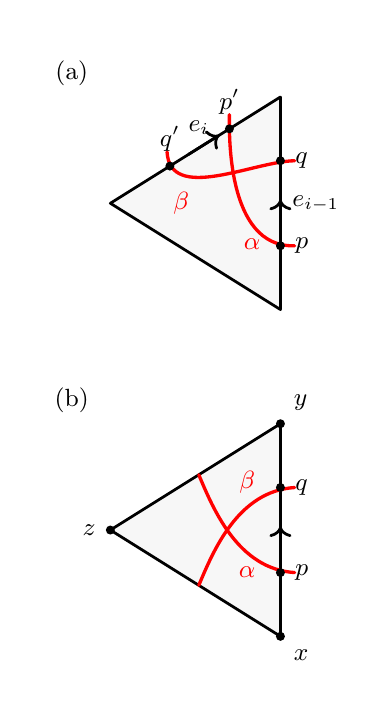
\begin{tikzpicture}[
  font=\small, line cap=round, line join=round,
  vertical diagram/.style={shift={(2.65,0)},rotate=90,scale=.9},
  point/.style={circle,fill=black,inner sep=1.15pt},
  note/.style={font=\scriptsize,align=center,text width=3.95cm,inner sep=0pt},
  heading/.style={font=\small,align=center}
]
\path[use as bounding box] (-.56,-4.65) rectangle (3.56,3.58);

\begin{scope}
  
  \node[heading] at (0,3) {(a)};
  \begin{scope}[vertical diagram]
  \fill[black!3] (0,0)--(3,0)--(1.5,2.4)--cycle;
  \draw[line width=1pt] (0,0)--(3,0)--(1.5,2.4)--cycle;
  \draw[line width=1pt, ->] (1.5,0)--(1.55,0);
  \draw[line width=1pt, ->] (2.19,1.296)--(2.46,.864);
  \draw[draw=red,line width=1.2pt] (.9,-0.2)..controls (.87,.78) and (2.55,.72)..(2.75,.72);
  \draw[draw=red,line width=1.2pt] (2.1,-0.2)..controls (2.09,.38) and (1.5,1.56)..(2.225,1.6);
  \node[text=red,below] at (1.13,0.4) {$\alpha$};
  \node[text=red,below] at (1.8,1.4) {$\beta$};
  \node[point,label=above:$p'$] at (2.55,.72) {};
  \node[point,label=above:$q'$] at (2.025,1.56) {};
  \node[label=$e_i$] at (2.2, 1.15) {};
  \node[label=$e_{i-1}$] at (1.1,-0.5) {};
  \node[point,label=right:$p$] at (.9,0) {};
  \node[point,label=right:$q$] at (2.1,0) {};
  \end{scope}
\end{scope}

\begin{scope}[yshift=-4.15cm]
  \node at (0,3) {(b)};
  \begin{scope}[vertical diagram]
  \fill[black!3] (0,0)--(3,0)--(1.5,2.4)--cycle;
  \draw[line width=1pt] (0,0)--(3,0)--(1.5,2.4)--cycle;
  \draw[line width=1pt, ->] (1.5,0)--(1.55,0);
  \draw[draw=red,line width=1.2pt] (.9,-0.2)..controls (.95,.6) and (1.8,.95)..(2.28,1.152);
  \draw[draw=red,line width=1.2pt] (2.1,-0.2)..controls (2.05,.6) and (1.2,.95)..(.72,1.152);
  \node[text=red,below] at (1.12,.47) {$\alpha$};
  \node[text=red,above] at (1.88,.47) {$\beta$};
  \node[point,label=below right:$x$] at (0,0) {};
  \node[point,label=above right:$y$] at (3,0) {};
  \node[point,label=left:$z$] at (1.5,2.4) {};
  \node[point,label=right:$p$] at (.9,0) {};
  \node[point,label=right:$q$] at (2.1,0) {};
  \end{scope}
\end{scope}

\end{tikzpicture}
\endgroup

\captionof{figure}{We assumed $\beta$ lies above $\alpha$ at $\vec{xy}$, but the definition of $\prec_L$ implies $\beta$ lies below $\alpha$ at an earlier triangle.}
\label{fig:crossing}
\end{minipage}\hfill
\begin{minipage}[t]{0.65\textwidth}
\setlength{\parskip}{0pt}
\setlength{\parindent}{\normalparindent}\indent
Starting from $p$, traverse $\alpha$ to the left of $\vec{e}$, and let $\vec{e}=\vec{e_1}, \vec{e_2}, \dots, \vec{e_r}$ be the sequence of oriented edges of the triangulation it meets. Note that $e_r$ is a boundary edge.  
Similarly, starting from $q$, traverse $\beta$ to the left and let $\vec{e}=\vec{f_1}, \vec{f_2}, \dots, \vec{f_s}$ be the sequence of oriented edges of the triangulation crossed by $\beta$.

Follow the curves $\alpha$ and $\beta$ as long as they intersect the same edges. Formally, let $I$ be the largest index such that $e_1=f_1,\dots,e_I=f_I$. For $i=1,\dots,I$, let $p_i$ and $q_i$ be the corresponding intersection points of $e_i=f_i$ with $\alpha$ and $\beta$, respectively.  Assume that for some  $i \geq 2$, we have that $q_i$ is closer to the start of $\vec{e_i}$ than $p_i$. Then for the first  such $i$, we have that $\alpha$ and $\beta$ cross while traversing from $e_{i-1}$ to $e_i$ (see Figure~\ref{fig:crossing} (a)).
Hence, we can assume that for each $i\leq I$, the point $p_i$ is closer to the start of $\vec{e_i}$ than $q_i$.

Now note that either the full sequences $e_1, \dots, e_r$ and $f_1, \dots, f_s$ are the same, or the curves $\alpha$ and $\beta$ separate after $e_I=f_I$. 
In the first case, $\alpha$ and $\beta$ must cross the same boundary edge $e_s$. But then $(\beta, q)\prec_L^{e} (\alpha, p)$ implies that $q_s$ is closer to the starting point of $\vec{e_s}$ than $p_s$, contradiction.

In the second case, let $xyz$ be the triangle to the left of $\vec{e_I}=\vec{xy}$.
Since $(\beta, q)\prec_L^{e}(\alpha, p)$, the curve $\beta$ exits $xyz$ through the edge $\vec{xz}$, while $\alpha$ exits it through $\vec{zy}$. However, this also means that $\alpha$ and $\beta$ must cross each other (see Figure~\ref{fig:crossing} (b)).\qedhere

\end{minipage}\par
\end{proof}

\subsection{Erd\H{o}s-Szekeres decompositions and the charging scheme.}

Recall that our proof of Theorem~\ref{thm:main} is based on a charging scheme --- we charge every curve to at least one oriented edge of triangle of $\cT$ such that no oriented edge or triangle is charged with more than $O(k^2)$ curves.
On a high level, the scheme works as follows.
At each oriented edge $\vec{xy}$, we assign to each $(\alpha, p) \in C_{xy}$ a successor, which is another curve $\beta$ crossing $xy$.
Then, looking at a curve $\alpha$, we charge it to each triangle at which its successor changes.
Since we have no parallel curves in $G$, such a successor change has to happen at some point for each curve $\alpha$. In order to define the notion of a successor, we introduce one further ingredient, which we call the Erd\H{o}s-Szekeres decomposition.

Let $S$ be an abstract set together with two linear orders, $\prec_L$ and $\prec_R$. 
An \emph{increasing subsequence} in $S$ is a sequence of elements of $S$ that is strictly increasing in both $\prec_L$ and $\prec_R$, and a \emph{decreasing subsequence} is a sequence that is strictly increasing in $\prec_L$, but decreasing in $\prec_R$. 
Each such set $S$ with orders $\prec_L, \prec_R$ naturally corresponds to a sequence of distinct real numbers, where $\prec_L$ orders the numbers by their position in the sequence, while $\prec_R$ orders the numbers by their size.

In the case of our drawing, at each oriented edge $\vec{xy}$, we consider $C_{xy}$ with the orders $\prec_L^{xy}$ and $\prec_R^{xy}$. We note that $C_{xy}$ does not contain a decreasing subsequence of length $k$, since by Lemma~\ref{lemma:comparability} it would correspond to $k$ pairwise crossing curves. The Erd\H{o}s-Szekeres theorem \cite{ESz} states that every sequence of $n$ distinct real numbers with no decreasing subsequence of length $k$ contains an increasing subsequence of length at least $n/(k-1)$. 
One of the most elegant proofs of this result, which is attributed to Seidenberg \cite{Seidenberg}, also provides a compact method to decompose such a sequence into a union of at most $k-1$ increasing subsequences.
This particular decomposition is crucial to our charging scheme and allows us to define the \emph{successor} of an element.

\begin{definition}
    Let $S$ be a set and $\prec_L,\prec_R$ two linear orders on $S$. For every $x\in S$, define 
    $$\ell_S(x)=\text{length of the longest decreasing subsequence ending with }x.$$
    The \emph{Erd\H{o}s-Szekeres decomposition} of $S$ is the partition of $S$ into sets
    $$L_S(i)=\{x\in S: \ell_S(x)=i\}\quad\text{for }i=1,2,\dots.$$
\end{definition}

\noindent
\begin{minipage}[t]{0.59\textwidth}
\vspace{0pt}
Each $L_S(i)$ is an increasing sequence in $S$. Given $x\in L_S(i)$, the \emph{successor} of $x$ in $S$ is defined as the successor of $x$ in $L_S(i)$. If $x$ is the last element of the sequence, it has no successor. See Figure \ref{fig:erdos-szekeres} for an illustration.

\smallskip

It is not hard to see that if $S$ contains no decreasing subsequence of length $k$, then the resulting Erd\H{o}s-Szekeres decomposition consists of at most $k-1$ non-empty sets, since $\ell_S(x)\leq k-1$ for all $x\in S$.
Thus, the Erd\H{o}s-Szekeres decomposition of $C_{xy}$ is composed of at most $k-1$ non-empty sets.
For each pair $(\alpha, p)$, we  define its \textit{successor at $\vec{xy}$} as its successor in $C_{xy}$ with respect to the orders $\prec_L^{xy}$ and $\prec_R^{xy}$. Now we are ready to define our charging scheme.

\end{minipage}\hfill
\begin{minipage}[t]{0.37\textwidth}
\vspace{0pt}\centering
\setlength{\captionindent}{0pt}
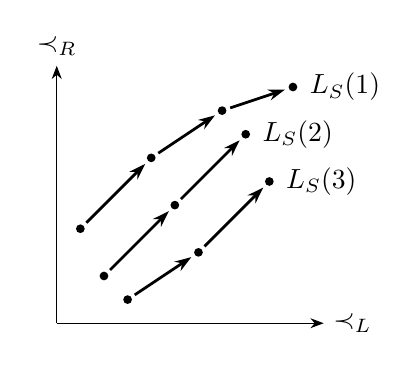
\begin{tikzpicture}[
    scale=0.3,
    transform shape,
    >=Stealth,
    draw=black, text=black,
    dot/.style={circle, fill=black, minimum size=10.5pt,
                inner sep=0pt, outer sep=5pt},
    chain/.style={-{Stealth[length=2.1mm,width=1.4mm]},
                  line width=1pt}
]
    \draw[->] (0,0) -- (11.3,0) node[transform shape=false,right] {$\prec_L$};
    \draw[->] (0,0) -- (0,10.9) node[transform shape=false,above] {$\prec_R$};

    \foreach \i/\p in {%
        1/4, 2/2, 3/1, 4/7, 5/5,
        6/3, 7/9, 8/8, 9/6, 10/10%
    } {
        \node[dot] (p\i) at (\i,\p) {};
    }

    \foreach \u/\v in {1/4,4/7,7/10,2/5,5/8,3/6,6/9}
        \draw[chain] (p\u) -- (p\v);
    \node[transform shape=false] at (12.2, 10) {$L_S(1)$};
    \node[transform shape=false] at (10.2, 8)  {$L_S(2)$};
    \node[transform shape=false] at (11.2, 6)  {$L_S(3)$};
\end{tikzpicture}
\captionof{figure}{\raggedright The Erd\H{o}s-Szekeres decomposition and the successors.}
\label{fig:erdos-szekeres}
\end{minipage}\par\medskip



\bigskip

\noindent
\textbf{Charging scheme.} Let $\alpha$ be a curve in our drawing. 
\begin{itemize}
    \item Let $\vec{xy}$ be an oriented edge of $\cT$. If there is a point $p\in \alpha\cap xy$ such that $(\alpha,p)$ has no successor at the edge $\vec{xy}$, then charge $\alpha$ to $\vec{xy}$. In this case, we say that $\alpha$ \emph{has no successor at $\vec{xy}$}.
    \item Let $xyz$ be a triangle of $\cT$, and assume that $\alpha$ crosses $xy$ and $xz$ in consecutive points $p$ and $q$. Then charge $\alpha$ to $xyz$ if
    \begin{itemize}
        \item  the successor of $(\alpha,p)$ at $\vec{xy}$ and the successor of $(\alpha,q)$ at $\vec{xz}$ come from different curves, or
        \item  the successor of $(\alpha,p)$ at $\vec{yx}$ and the successor of $(\alpha,q)$ at $\vec{zx}$ come from different curves.
    \end{itemize}
    If $\alpha$ is charged to $xyz$, we say that $\alpha$ \emph{switches successors in $xyz$}.
\end{itemize}

\medskip

We now argue that every curve is charged to at least one oriented edge or triangle, and that no oriented edge or triangle is charged with too many curves.

\begin{lemma}\label{lemma:charging_curves}
Every curve $\alpha$ is charged to at least one oriented edge or triangle of $\cT$. 
\end{lemma}
\begin{proof}
Traverse $\alpha$ from one endpoint to the other, and let $e_1, \dots, e_s$ be the sequence of edges of $\cT$ crossed by $\alpha$ in order, and let $p_1, \dots, p_s$ be the corresponding crossing points. Note that $e_1$ and $e_s$ are boundary edges. Orient each edge $e_i$ as $\vec{e_i}$ such that $\alpha$ crosses from right-to-left.

Assume that $(\alpha,p_i)$ has a successor at every edge $e_i$, as otherwise $\alpha$ is charged to some oriented edge. Moreover, if for some $i$, the successors of $(\alpha, p_i)$ and $(\alpha,p_{i+1})$ at $e_i$ and $e_{i+1}$ come from different curves, then $\alpha$ is charged to the triangle whose sides are $e_i$ and $e_{i+1}$. 

So, if $\alpha$ is not charged at any step, its successor at both boundary edges $e_1$ and $e_s$ must correspond to the same curve, say $\beta$. But then $\alpha$ and $\beta$ are parallel edges in the graph $G$, contradicting the fact that $G$ is a simple graph.
\end{proof}

The final step of the proof is showing that at most $O(k^2)$ curves are charged to any given triangle, and $O(k)$ curves are charged to any edge. To this end, we wish to understand how the Erd\H{o}s-Szekeres decompositions for two oriented edges, say $\vec{xy}$ and $\vec{xz}$, of the same triangle differ.

Let $S'$ be a set with linear orders $\prec_L, \prec_R$ and let $S\subseteq S'$ be its subset, ordered with the same linear orders. Define
$$\cD(S,S')=\#\{x\in S:\text{ the successor of $x$ in $S$ is different from its successor in $S'$}\}.$$
If an element $x$ has no successor in $S$, but has one in $S'$, it is also included in $\cD(S, S')$. Similarly, if $x$ has no successor in $S'$, but has one in $S$, it is also included. The following lemma bounds the maximum number of successor changes that may occur if we restrict to certain special subsets of~$S'$, see Figure~\ref{fig:successor-changes} for an illustration.

\begin{lemma}\label{lemma:erdos-szekeres}
Let $S\subseteq S'$, and let $\prec_L, \prec_R$ be two linear orders on $S'$, such that there is no decreasing sequence of length $k$ in $S'$.
\begin{enumerate}
  \item Assume $S$ is the set of $|S|$ smallest elements in $S'$ under $\prec_R$. Then $\cD(S, S') \leq \binom{k}{2}$.

  \item Assume $S$ is the set of $|S|$ largest elements in $S'$ under $\prec_R$. Then $\cD(S, S') =0$.
  
  \item Assume $S$ is the set of first $|S|$ elements in $S'$ under $\prec_L$. Then $\cD(S, S')\leq k-1$.

  \item Assume $S$ is the set of last $|S|$ elements in $S'$ under $\prec_L$. Then $\cD(S, S') \leq \binom{k}{2}$.
\end{enumerate}
\end{lemma}
\vspace{-0.4cm}
\begin{figure}[htbp]
\centering

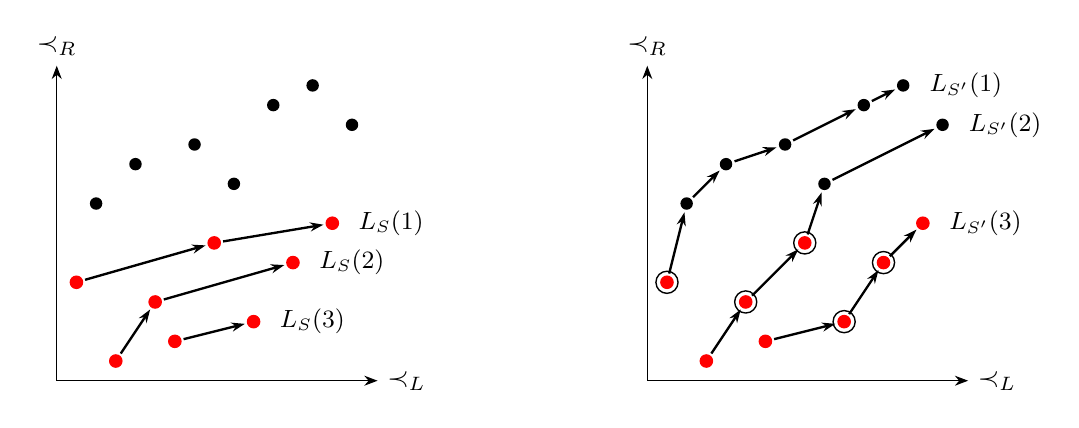
\begin{tikzpicture}[
    scale=0.25,
    >=Stealth,
    draw=black, text=black,
    dot/.style={circle, fill=black, minimum size=4.5pt,
                inner sep=0pt, outer sep=1pt},
    chain/.style={-{Stealth[length=1.7mm,width=1.15mm]},
                  line width=0.85pt},
    chainlabel/.style={anchor=west, xshift=6pt, font=\small}
]
    \begin{scope}[shift={(0,0)}]
        \draw[->] (0,0) -- (16.3,0) node[right] {$\prec_L$};
        \draw[->] (0,0) -- (0,16) node[above] {$\prec_R$};

        \foreach \i/\p in {1/5,2/9,3/1,4/11,5/4,6/2,7/12,8/7,9/10,10/3,11/14,12/6,13/15,14/8,15/13} {
            \ifnum\p<9\relax
                \node[dot, fill=red, draw=red] (s\i) at (\i,\p) {};
            \else
                \node[dot] (s\i) at (\i,\p) {};
            \fi
        }

        \foreach \u/\v in {1/8,8/14}
            \draw[chain] (s\u) -- (s\v);

        \foreach \u/\v in {3/5,5/12}
            \draw[chain] (s\u) -- (s\v);

        \foreach \u/\v in {6/10}
            \draw[chain] (s\u) -- (s\v);

        \node[chainlabel] at (s14) {$L_{S}(1)$};
        \node[chainlabel] at (s12) {$L_{S}(2)$};
        \node[chainlabel] at (s10) {$L_{S}(3)$};
    \end{scope}

    \begin{scope}[shift={(30,0)}]
        \draw[->] (0,0) -- (16.3,0) node[right] {$\prec_L$};
        \draw[->] (0,0) -- (0,16) node[above] {$\prec_R$};

        \foreach \i/\p in {1/5,2/9,3/1,4/11,5/4,6/2,7/12,8/7,9/10,10/3,11/14,12/6,13/15,14/8,15/13} {
            \ifnum\p<9\relax
                \node[dot, fill=red, draw=red] (p\i) at (\i,\p) {};
            \else
                \node[dot] (p\i) at (\i,\p) {};
            \fi
        }

        \foreach \u/\v in {1/2,2/4,4/7,7/11,11/13}
            \draw[chain] (p\u) -- (p\v);

        \foreach \u/\v in {3/5,5/8,8/9,9/15}
            \draw[chain] (p\u) -- (p\v);

        \foreach \u/\v in {6/10,10/12,12/14}
            \draw[chain] (p\u) -- (p\v);

        \node[chainlabel] at (p13) {$L_{S'}(1)$};
        \node[chainlabel] at (p15) {$L_{S'}(2)$};
        \node[chainlabel] at (p14) {$L_{S'}(3)$};

        \foreach \i in {1,5,8,10,12} {
    \node[
        circle,
        draw=black,
        fill=none,
        minimum size=8pt,
        inner sep=0pt,
        outer sep=0pt,
        line width=0.5pt
    ] at (p\i) {};
}
    \end{scope}
\end{tikzpicture}
\caption{An illustration of the Erd\H{o}s-Szekeres decompositions of $S$ and $S'$ in case (1), where the red points denote the elements of $S$. The circled elements have different successors in $S$ and $S'$.}
\label{fig:successor-changes}
\end{figure}


We postpone the proof of Lemma~\ref{lemma:erdos-szekeres} to the next subsection.
Here, we  finish the analysis of our charging scheme, by showing that each oriented edge and triangle is charged with at most $O(k^2)$ curves.
\begin{lemma}\label{lemma:charging_edges}
\begin{enumerate}
  \item[(a)] An oriented edge $\vec{xy}$ of $\cT$ is charged with at most $k-1$ curves.
  \item[(b)] A triangle $xyz$ of $\cT$ is charged with at most $6k^2$ curves.
\end{enumerate}
\end{lemma}
\begin{proof}
\textit{(a)} The oriented edge $\vec{xy}$ is charged with $\alpha$ if there is some $p\in \alpha\cap xy$ such that $(\alpha, p)$ is the largest element of one of the increasing sequences given by the Erd\H{o}s-Szekeres decomposition. There are at most $k-1$ sequences in this decomposition, so this finishes the proof.

\medskip
\textit{(b)} Recall that $xyz$ is charged with a curve $\alpha$ if for some $$(e,f)\in \{(xy,xz),(yx,zx),(yx,yz),(xy,zy),(xz,yz),(zx,zy)\}$$
the curve $\alpha$ crosses $e$ and $f$ in some consecutive points $p$ and $q$, respectively, such that the successor of $(\alpha,p)$ at $\vec{e}$ comes from a different curve than the successor of $(\alpha,q)$ at $\vec{f}$. It suffices to show that a triangle is charged with at most $k^2$ curves for each of the six listed pairs. By symmetry, it suffices to analyze only two cases, namely when $(e,f)=(xy,xz)$ and $(e, f)=(yx, zx)$ (see Figure~\ref{fig:charging-triangle}).

First, let $(e, f)=(xy, xz)$, and assume that the triangle $xyz$ is to the left of $\vec{xy}$, as otherwise we can switch $y$ and $z$. Let $S$ be the set of triples $(\alpha, p, q)$ for which the curve $\alpha$ joins the points $p\in xy\cap \alpha$ and $q\in xz\cap \alpha$ without exiting the triangle $xyz$. Then $S$ can be naturally identified with subsets of both $C_{xy}$ and $C_{xz}$.

\begin{figure}[htbp]
\centering
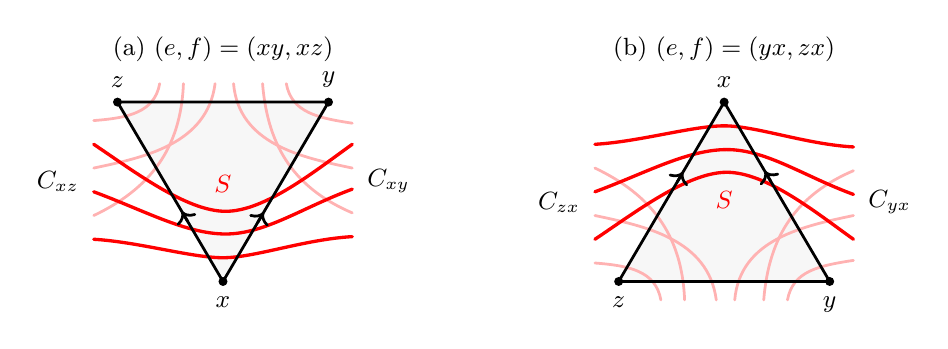
\begin{tikzpicture}[scale=.67, line cap=round, line join=round, font=\small,
  point/.style={circle,fill=black,inner sep=1.15pt},
  curve/.style={draw=red,line width=1.2pt},
  othercurve/.style={draw=red!30,line width=1pt},
  heading/.style={font=\small,align=center}]
\def\cornerpicture{%
  \fill[black!3] (2,0)--(4,3.4)--(0,3.4)--cycle;
  \draw[othercurve] (-.45,1.25)..controls (.6,1.75) and (1.2,2.5)..(1.25,3.75);
  \draw[othercurve] (-.45,2.15)..controls (.5,2.35) and (1.7,2.6)..(1.85,3.75);
  \draw[othercurve] (-.45,3.05)..controls (.2,3.1) and (.7,3.2)..(.8,3.75);
  \draw[othercurve] (4.45,1.3)..controls (3.4,1.75) and (2.85,2.5)..(2.75,3.75);
  \draw[othercurve] (4.45,2.15)..controls (3.5,2.35) and (2.3,2.6)..(2.2,3.75);
  \draw[othercurve] (4.45,3.0)..controls (3.8,3.1) and (3.3,3.2)..(3.2,3.75);
  \draw[curve] (-.45,.8)..controls (.4,.75) and (1.4,.45)..(2,.45)
    ..controls (2.6,.45) and (3.55,.8)..(4.45,.85);
  \draw[curve] (-.45,1.7)..controls (.5,1.35) and (1.3,.9)..(2.05,.9)
    ..controls (2.8,.9) and (3.5,1.4)..(4.45,1.75);
  \draw[curve] (-.45,2.6)..controls (.3,2.1) and (1.3,1.33)..(2.05,1.33)
    ..controls (2.8,1.33) and (3.75,2.1)..(4.45,2.6);
  \draw[line width=1pt] (2,0)--(4,3.4)--(0,3.4)--cycle;
  \node[text=red] at (2,1.85) {$S$};
}
\begin{scope}
  \node[heading] at (2,4.4) {(a) $(e,f)=(xy,xz)$};
  \cornerpicture
  \draw[line width=1pt,->] ($(2,0)!.33!(4,3.4)$)--($(2,0)!.385!(4,3.4)$);
  \draw[line width=1pt,->] ($(2,0)!.335!(0,3.4)$)--($(2,0)!.39!(0,3.4)$);
  \node[point,label=below:$x$] at (2,0) {};
  \node[point,label=above:$y$] at (4,3.4) {};
  \node[point,label=above:$z$] at (0,3.4) {};
  \node[anchor=west] at (4.55,1.9) {$C_{xy}$};
  \node[anchor=east] at (-.55,1.9) {$C_{xz}$};
\end{scope}
\begin{scope}[xshift=9.5cm]
  \node[heading] at (2,4.4) {(b) $(e,f)=(yx,zx)$};
  \begin{scope}[yshift=3.4cm,yscale=-1]
    \cornerpicture
  \end{scope}
  \draw[line width=1pt,->] ($(2,3.4)!.44!(4,0)$)--($(2,3.4)!.385!(4,0)$);
  \draw[line width=1pt,->] ($(2,3.4)!.445!(0,0)$)--($(2,3.4)!.39!(0,0)$);
  \node[point,label=above:$x$] at (2,3.4) {};
  \node[point,label=below:$y$] at (4,0) {};
  \node[point,label=below:$z$] at (0,0) {};
  \node[anchor=west] at (4.55,1.5) {$C_{yx}$};
  \node[anchor=east] at (-.55,1.5) {$C_{zx}$};
\end{scope}
\end{tikzpicture}
\caption{The two cases in the proof of Lemma~\ref{lemma:charging_edges}(b). The set $S$ consists of highlighted curves, which connect $xy$ to $xz$. The orders of $xy$ and $xz$ agree on $S$.}
\label{fig:charging-triangle}
\end{figure}

Our goal is now to count the number of triples $(\alpha, p, q)\in S$ for which the successors of $(\alpha, p)$ at $xy$ and $(\alpha, q)$ at $xz$ come from different curves. From their definition, we see that the orders $\prec_L^{xy}, \prec_R^{xy}$ agree with $\prec_L^{xz}, \prec_R^{xz}$ on $S$. Under this identifications, the successors in the decomposition of $S$ on the two edges $xy, xz$ agree.

Note that $S$ is the set of first $|S|$ elements in $C_{xy}$ under $\prec_L^{xy}$ (this is illustrated in Figure~\ref{fig:charging-triangle}, since the edges of $S$ have the left endpoint ``below'' the other curves intersecting $xy$). Hence, (3) in Lemma \ref{lemma:erdos-szekeres} implies that $\cD(S,C_{xy})\leq k-1$. Similarly, $S$ is the set of smallest $|S|$ elements in $C_{xz}$ under $\prec_R^{xz}$, and so (1) in Lemma \ref{lemma:erdos-szekeres} implies that $\cD(S,C_{xz})\leq \binom{k}{2}$. Thus, the number of elements of $S$ with different successors in $C_{xy}$ and $C_{xz}$ is at most $\cD(S,C_{xy})+\cD(S,C_{xz})\leq \binom{k}{2}+k-1\leq k^2$.

The argument proceeds very similarly when $(e, f)=(yx, zx)$. Assuming now that $xyz$ is to the left of $\vec{yx}$, we define $S$ as before, and observe that it is a subset of both $C_{yx}$ and $C_{zx}$. In this case, $S$ is the set of last $|S|$ elements in $C_{yx}$ under $\prec_L^{yx}$, and therefore (4) in Lemma~\ref{lemma:erdos-szekeres} implies that $\cD(S, C_{yx})\leq \binom{k}{2}$. On the other hand, $S$ is also the set of largest $|S|$ elements in $C_{zx}$ under $\prec_R^{zx}$, and therefore (2) in Lemma~\ref{lemma:erdos-szekeres} shows that $\cD(S, C_{zx})=0$. This is illustrated in Figure~\ref{fig:charging-triangle}(b). Hence, the number of elements of $S$ with different successors in $C_{yx}$ and $C_{zx}$ is at most $\cD(S,C_{yx})+\cD(S,C_{zx})\leq \binom{k}{2}+0\leq k^2$.
\end{proof}

Combining Lemma~\ref{lemma:charging_curves} with Lemma~\ref{lemma:charging_edges} immediately implies Theorem~\ref{thm:main}.

\subsection{Bounding the number of successor changes}
The only remaining bit is hence to prove Lemma~\ref{lemma:erdos-szekeres}.
The proof is slightly technical, but the main idea is to simply look at how the lengths of the longest decreasing sequences $\ell_{S}(x)$ and $\ell_{S'}(x)$ can differ in each of the cases.

\begin{proof}[Proof of Lemma~\ref{lemma:erdos-szekeres}.]
We consider the four cases individually. Recall that for $x\in S$, $\ell_S(x)$ denotes the length of the longest decreasing sequence in $S$ ending with $x$. Throughout the proof, we think of $S, S'$ as sequences, where $x$ comes before $y$ if $x\prec_L y$.

\bigskip
\noindent
\textit{(1)} We begin with two preparatory claims. First, we claim that if $x$ comes before $y$ in $S$ and both belong to the same increasing sequence in the decomposition of $S$, i.e. $\ell_S(x)=\ell_S(y)$, then $\ell_{S'}(x) \leq \ell_{S'}(y)$.
    
Assume for contradiction that there exist $x,y\in S$ violating this statement.
Among all such pairs $(x,y)$, choose one that minimizes $\ell=\ell_S(x)$.
Let $L$ be a decreasing subsequence of $S'$ of length $\ell_{S'}(x)$ ending at $x$.
Note that if all elements of $L\setminus\{x\}$ are in $S'\setminus S$, then replacing $x$ by $y$ in the sequence $L$ yields a decreasing subsequence of length $\ell_{S'}(x)$ ending at $y$, giving $\ell_{S'}(x) \leq \ell_{S'}(y)$. Let $x'$ be the element of $L$ preceding $x$, then $x'\in S$. If $y\prec_R x'$, then replacing $x$ with $y$ in $L$ would again yield a decreasing subsequence of length $\ell_{S'}(x)$, so we must have $x'\prec_R y$.
Moreover, $\ell_S(x')<\ell_S(x)=\ell$. Let $y'\in S$ be such that $\ell_S(y') = \ell_S(x')$ and $y'$ lies on a decreasing subsequence of length $\ell_S(y)$ ending at $y$ in $S$. As $x'\prec_R y\prec_R y'$, we have $x'\prec_R y'$. By the minimality of $\ell$, we must have $\ell_{S'}(y') \geq \ell_{S'}(x') = \ell_{S'}(x) - 1$, and hence $\ell_{S'}(y) \geq \ell_{S'}(y') + 1 \geq \ell_{S'}(x)$, a contradiction.
\medskip

Next, we state and prove our second claim. It states that if $x$ comes before $y$ in $S$ and $\ell_{S'}(x)=\ell_{S'}(y)$, then $\ell_{S}(y) \leq \ell_{S}(x)$.

Assume for contradiction that for some $x$ preceding $y$ in $S$, we have $\ell_{S'}(x) = \ell_{S'}(y)$ and $\ell_S(x) < \ell_S(y)$.
Consider a decreasing subsequence of $S$  of length $\ell_S(y)$ ending at $y$, and let $y'$ be an element of this sequence such that $\ell_S(y')=\ell_S(x)$.
We have $x\prec_R y\prec_R y'$, and thus $y'$ lies between $x$ and $y$ in the sequence.
Then, by the previous claim, we get $\ell_{S'}(y') \geq \ell_{S'}(x)$, and therefore
    $\ell_{S'}(y) \geq  \ell_{S'}(y') + 1 > \ell_{S'}(x),$
a contradiction.

Consider $L_S(\ell)$, i.e. the increasing sequences in the decomposition of $S$ composed of elements $x\in S$ such that $\ell_S(x)=\ell$. Let $x_1, \dots, x_p$ be the elements of $L_S(\ell)$ which have different successors in $S$ and $S'$.
We claim that 
\begin{equation*}
\hspace{4cm}\ell \leq \ell_{S'}(x_1) < \ell_{S'}(x_2) < \dots < \ell_{S'}(x_p) \leq k-1.\hspace{4cm} (*)
\end{equation*}
    
The first of these inequalities follows since $\ell_{S'}(x_1) \geq \ell_S(x_1) = \ell$, while the last one $\ell_{S'}(x_p) \leq k-1$ follows since $S'$ contains no decreasing subsequence of length $k$.

Hence, it remains to prove that for $1\leq i < p$, we have $\ell_{S'}(x_i) < \ell_{S'}(x_{i+1})$. Let $y$ be the successor of $x_i$ in $S$. By the first claim applied to the pairs $(x_i, y)$ and $(y, x_{i+1})$ (noting that both pairs satisfy the assumptions of the claim by definition), we have $\ell_{S'}(x_{i+1})\geq \ell_{S'}(y)\geq \ell_{S'}(x_i)$, so it suffices to show that $\ell_{S'}(y)>\ell_{S'}(x_i)$.

Suppose we had $\ell_{S'}(y)=\ell_{S'}(x_i)$. If $y'\neq y$ is the successor of $x_i$ in $S'$, then $y'$ is between $x_i$ and $y$ in the sequence $S'$ and has $\ell_{S'}(x_i)=\ell_{S'}(y')$. So, $y$ and $y'$ are in the same increasing sequence of $S'$, and we would have $y'\prec_R y$. As $S$ is the set of $|S|$ smallest elements under $\prec_R$, this implies $y'\in S$.

Applying the second claim to the pairs $(x_i, y')$ and $(y', y)$ then shows that $\ell_{S}(y') \leq \ell_S(x_i)$ and $\ell_S(y)\leq \ell_S(y')$. As $\ell_S(x_i)=\ell_S(y)$, this quantity equals $\ell_S(y')$, which means that $y'$ is in the same increasing sequence of $S$ as $x_i$ and $y$. But then $y$ cannot be the successor of $x_i$ in $S$, contradiction.

We proved that in $L_S(\ell)$, there are $p \leq k - \ell$ elements whose successor is changed. Thus, the statement of \textit{(1)} is then immediately obtained by summing over $\ell=1, \dots, k-1$, i.e. $\cD(S,S')\leq (k-1)+\dots+1=\binom{k}{2}$. 


\bigskip
\noindent
\textit{(2)} Clearly, we have $\ell_S(x) = \ell_{S'}(x)$ for all $x \in S$ as no decreasing subsequence ending at $x$ can contain an element from $S' \setminus S$. Moreover, for every $x \in S$ and  $y \in S' \setminus S$ such that $x$ precedes $y$, we have $\ell_{S'}(y) \geq \ell_S(x) + 1$, as we can append $y$ to every decreasing subsequence ending at $x$. This implies that all $x \in S$ have the same successor in both $S$ and $S'$.

\bigskip
\noindent
\textit{(3)} As in the previous case, we have $\ell_S(x) =  \ell_{S'}(x)$ for all $x \in S$ as these value do not depend on elements $y\in S'$ for which $x$ precedes $y$. It immediately follows that every $x \in S$ that has a successor in $S$ has the same successor in $S'$. Only the elements of $S$ with no successor in $S$ can gain a successor in $S'$, showing that $\cD(S,S')\leq k-1$.

\bigskip
\noindent
\textit{(4)} We show that (1) implies (4) by a symmetry argument.

Let $\lhd_L$ be the reverse of $\prec_R$, and let $\lhd_R$ be the reverse of $\prec_L$ on $S'$. To minimize confusion, we denote by $T, T'$ the sets $S, S'$ when they are ordered using the orders $\lhd_L, \lhd_R$. Observe that reversing an increasing sequence with respect to $\prec_L, \prec_R$ gives an increasing sequence in $\lhd_L, \lhd_R$. On the other hand, a decreasing sequence with respect to orders $\prec_L, \prec_R$ remains decreasing with respect to orders $\lhd_L, \lhd_R$. In particular, for every element $x$, the length of the longest decreasing sequence ending at $x$ is unchanged, i.e. $\ell_S(x)=\ell_T(x)$ and $\ell_{S'}(x)=\ell_{T'}(x)$. Hence, the successor of $x$ in $T$ (or $T'$) is the predecessor of $x$ in $S$ (or $S'$). The \textit{predecessor} of $x$ is the element immediately before it in its increasing sequence in the Erd\H{o}s-Szekeres decomposition.

The main advantage of this transformation is that $T$ is now the set of smallest $|T|$ elements in $T'$ under $\lhd_R$, which corresponds to the situation of (1). 
To bound $\cD(S, S')$, we bound the number of elements $x\in T$ with different predecessors in $T$ and $T'$. If the starting elements of the increasing sequences are the same in $T$ and $T'$, then the number of $x\in T$ whose predecessor changes is at most $\cD(T, T')$ (which is at most $ \binom{k}{2}$ by (1)). 
The reason is simple: if $x'$ was the predecessor of $x$ in $T$, but is not in $T'$, then the successor of $x'$ must have changed from $T$ to $T'$. 

To ensure that the increasing sequences in both $T$ and $T'$ start with the same elements, add to the start of both sequences a set $A$ consisting of $k-1$ dummy elements with $a_{k-1}\lhd_R \dots\lhd_R a_{1}$ and $a_1\lhd_L a_2\lhd_L\dots\lhd_L a_{k-1}$, such that $a_i\lhd_R x$ and $a_i\lhd_L x$ for all $a_i\in A, x\in T'$. A dummy and a real element cannot be in the same decreasing sequence, and so the increasing sequences in both $T$ and $T'$ start with $a_1, \dots, a_{k-1}$. Therefore, $\cD(S, S')\leq \cD(A\cup T, A\cup T')\leq \binom{k}{2}$, where the last inequality follows from (1), since $A\cup T$ is the set of smallest $|A|+|T|$ elements in $A\cup T'$ under $\lhd_R$.
\end{proof}   

\section*{AI declaration}

The AI tools were used for understanding the paper of Beeker and Lazarovich \cite{BL}. The main new idea of this work, to consider the orders $\prec_L, \prec_R$ and the resulting Erd\H{o}s-Szekeres decomposition is due to the authors. Once provided with this idea and the statement of Lemma~\ref{lemma:erdos-szekeres}, AI tools assisted in the proof of Lemma \ref{lemma:erdos-szekeres}. 

\vspace{-0.1cm}
\begin{thebibliography}{99}
\bibitem{Ackerman}
E. Ackerman.
\emph{On the maximum number of edges in topological graphs with no four
pairwise crossing edges.}
Discrete Comput. Geom. 41 (2009): 365--375.

\bibitem{AT}
E. Ackerman, and G. Tardos.
\emph{On the maximum number of edges in quasi-planar graphs.}
J. Combin. Theory Ser. A 114(3) (2007): 563--571.

\bibitem{AAPPS}
P. K. Agarwal, B. Aronov, J. Pach, R. Pollack and M. Sharir.
\emph{Quasi-planar graphs have a linear number of edges.}
Combinatorica 17 (1997): 1--9.

\bibitem{AEGKKPS}
B. Aronov, P. Erd\H{o}s, W. Goddard, D.J. Kleitman, M. Klugerman, J. Pach, and L.J. Schulman. \emph{Crossing families.}
Combinatorica 14 (2) (1994): 127--134.

\bibitem{BL}
B. Beeker, and N. Lazarovich.
\emph{Cubical accessibility and bounds on curves on surfaces.}
Journal of Topology 10 (2017): 1050--1065.

\bibitem{Brandenburg}
J. F. Brandenburg.
\emph{A simple quasi-planar drawing of $K_{10}$.}
In Graph Drawing, vol. 9801 (2016): 603--604.

\bibitem{BMP}
P. Brass, W. Moser, and J. Pach. 
\emph{Research Problems in Discrete Geometry.}
Berlin, Germany, Springer-Verlag, 2005.

\bibitem{CP}
V. Capoyleas, and J. Pach.
\emph{A Tur\'an-type theorem on chords of a convex polygon.}
J. Comb. Theory Ser. B 56 (1992): 9--15.

\bibitem{ESz}
P. Erd\H{o}s, and G. Szekeres.
\emph{A combinatorial problem in geometry.}
Compositio Mathematica 2 (1935): 463--470.

\bibitem{Fary}
I. F\'ary.
\emph{On straight-line representation of planar graphs}
Acta Sci. Math. (Szeged), 11 (1948): 229--233.

\bibitem{FP}
J. Fox, and J. Pach. 
\emph{Applications of a new separator theorem for string graphs.}
Combin. Probab. Comput. 23 (2014): 66--74.

\bibitem{FPS}
J. Fox, J. Pach, and A. Suk.
\emph{Quasiplanar graphs, string graphs, and the Erd\H{o}s-Gallai problem.}
European Journal of Combinatorics 119 (2024): 103811.

\bibitem{PRT}
J. Pach,  N. Rubin, and G. Tardos. 
\emph{Planar point sets determine many pairwise crossing segments.}
Advances in Mathematics 386 (2021): 107779.

\bibitem{PSSz}
J. Pach, F. Shahrokhi, and M. Szegedy.
\emph{Applications of the crossing number.}
J. Graph Theory 22 (1996): 239--243.

\bibitem{PTZ}
J. Pach, G. Tardos, and J. Zeng.
\emph{On the number of edges in quasiplanar graphs.}
preprint, arXiv:2611.07314 (2026)

\bibitem{Sadhu}
A. Sadhu.
\emph{Every $k$-Quasi-Planar Graph Has Linearly Many Edges.}
preprint, arXiv:2611.01509 (2026)

\bibitem{Seidenberg}
 A. Seidenberg.
 \emph{A simple proof of a theorem of Erd\H{o}s and Szekeres.}
 Journal of the London Mathematical Society, 34 (3) (1959): 352.

\bibitem{Toth}
G. T\'oth.
\emph{Note on Geometric Graphs.}
Journal of Combinatorial Theory, Series A 89 (2000): 126--132.

\bibitem{Valtr}
P. Valtr. 
\emph{Graph drawing with no $k$ pairwise crossing edges.}
International Symposium on Graph Drawing. Berlin, Heidelberg: Springer Berlin Heidelberg, 1997.

\bibitem{Valtr2}
P. Valtr.
\emph{On geometric graphs with no $k$ pairwise parallel edges.}
Discrete Comput. Geom. 19 (1998): 461--469.

\end{thebibliography}

\end{document}